\chapter[Electrical Power Balance and Battery Model]
{Electrical Power Balance\\and Battery Model}
\label{ch:electrical_battery_analysis}

The \texttt{Energy balance} tab extends the thermal post-processing workflow
with a separate electrical calculation. The module first uses the solar load
exported by \acrshort{esatan-tms} to estimate the power generated by the solar
cells. It then obtains the electrical demand from the internal dissipations of
the selected equipment and applies the resulting power surplus or deficit to a
configurable lithium-ion battery model.

All operations take place after the thermal solution. The application reads
$Q_S$, $Q_I$ and the required temperature histories from the imported
\texttt{.TMD} file, but it does not modify those data or return any electrical
quantity to \acrshort{esatan-tms}. The thermal and electrical calculations
therefore remain one-way coupled: the solved thermal case supplies the inputs,
and the Python module derives solar generation, electrical demand, battery
state and operating limits.

The workflow contains two consecutive stages. The first converts the selected
solar-panel result into $Q_{S,\mathrm{elec}}$ and builds
$Q_{\mathrm{load}}$. The second uses both histories, together with the
battery temperature and the configurable cell parameters, to calculate stored
energy, state of charge, terminal voltage, charge and discharge currents,
losses and operating phases.


\section{Solar-to-Electrical Power Conversion}
\label{sec:solar_electrical_conversion}

\subsection{Conversion Method}
\label{subsec:solar_conversion_method}

The selected solar-panel group provides the absorbed solar load $Q_S(t)$. In
the adopted thermo-electrical formulation, the incident solar power
$Q_{S,i}(t)$ divides into a thermal fraction and an electrical fraction. The
solar absorptivity $\alpha$ describes the total fraction retained by the solar
cells, while the electrical conversion efficiency $\eta(t)$ defines the part
converted into electrical power. The effective thermal absorptivity becomes

\begin{equation}
    \alpha_{\mathrm{th}}(t)
    =
    \alpha-\eta(t).
    \label{eq:solar_effective_absorptivity}
\end{equation}

The thermal load exported for the selected group follows

\begin{equation}
    Q_S(t)
    =
    \left[\alpha-\eta(t)\right]Q_{S,i}(t).
    \label{eq:solar_thermal_load_conversion}
\end{equation}

The application therefore reconstructs the incident power from

\begin{equation}
    Q_{S,i}(t)
    =
    \frac{Q_S(t)}{\alpha-\eta(t)},
    \label{eq:solar_incident_power_reconstruction}
\end{equation}

and calculates the electrical contribution as

\begin{equation}
    Q_{S,\mathrm{elec}}(t)
    =
    \eta(t)Q_{S,i}(t)
    =
    \frac{\eta(t)}{\alpha-\eta(t)}Q_S(t).
    \label{eq:solar_electrical_power}
\end{equation}

The calculation requires
$0<\eta(t)<\alpha\leq 1$ throughout the simulated interval. The user may
introduce $\eta$ as a constant or as a function of the mean temperature of the
selected solar-panel element. A temperature-dependent expression therefore
has the general form

\begin{equation}
    \eta(t)
    =
    f_{\eta}\!\left[T_{\mathrm{SP,mean}}(t)\right].
    \label{eq:solar_efficiency_temperature_function}
\end{equation}

This option allows the conversion efficiency to follow the thermal result
without requiring a complete current--voltage or maximum-power-point model.
When the user enters a constant, the same value applies to every output
instant.

The electrical demand comes from the internal dissipations of the selected
consumer groups. For the set of load elements $\mathcal{G}_{\mathrm{load}}$,
the application calculates

\begin{equation}
    Q_{\mathrm{load}}(t)
    =
    \sum_{g\in\mathcal{G}_{\mathrm{load}}}
    \max\!\left[Q_{I,g}(t),0\right].
    \label{eq:electrical_load_from_qi_ch8}
\end{equation}

This approximation treats the positive internal load of each selected unit as
its electrical consumption. It suits the electronic equipment represented in
the model, for which most of the consumed power finally appears as heat. The
method does not separately account for exported mechanical work,
radio-frequency power or conversion losses outside the battery model.

The difference between generation and demand defines the power available
before battery operation:

\begin{equation}
    P_{\mathrm{net}}(t)
    =
    Q_{S,\mathrm{elec}}(t)-Q_{\mathrm{load}}(t).
    \label{eq:electrical_net_power_ch8}
\end{equation}

Positive values provide solar surplus for charging, whereas negative values
require battery discharge. The corresponding non-negative magnitudes are

\begin{align}
    P_{\mathrm{sur}}(t)
    &=
    \max\!\left[P_{\mathrm{net}}(t),0\right],
    \label{eq:solar_surplus_ch8}
    \\
    P_{\mathrm{def}}(t)
    &=
    \max\!\left[-P_{\mathrm{net}}(t),0\right].
    \label{eq:load_deficit_ch8}
\end{align}

Solar generation always supplies the load first. The battery only receives the
remaining surplus or covers the remaining deficit.


\subsection{Input Selection and Electrical-Balance Display}
\label{subsec:solar_balance_configuration}

The upper area of the tab gathers the inputs required by the previous
relations. The user first selects a transient case and defines the efficiency
through the \emph{$\eta$ equation or constant} field. When the expression
contains $T$, the application evaluates it with the mean temperature of the
selected solar-panel element in degrees Celsius. The solar conversion does not
use terminal voltage as an efficiency variable.

The \emph{Elements} selector lists the hierarchy groups with a non-zero
$Q_S$ history. The chosen group identifies the solar-panel nodes whose load
enters Equation~\eqref{eq:solar_incident_power_reconstruction}. The
\emph{$Q_{\mathrm{load}}$ elements} selector then lists the groups with a
non-zero $Q_I$ contribution. The application sums every selected group, so the
user must avoid choosing a parent group together with one of its descendants
when both contain the same nodes. Such a selection would count the same
internal dissipation twice.

The thermo-optical selector retrieves the solar absorptivity from the property
sets contained in the imported results. When the required set is unavailable
or the user needs another value, the interface accepts manual values of
$\alpha$ and $\varepsilon$. The current conversion uses $\alpha$;
$\varepsilon$ remains stored with the analysis to preserve the selected
thermo-optical definition.

Figure~\ref{fig:solar_electrical_configuration} shows the configuration area.
The layout follows the calculation sequence: efficiency, solar element,
electrical-load elements, thermo-optical properties and output curves.

\begin{figure}[H]
    \centering
    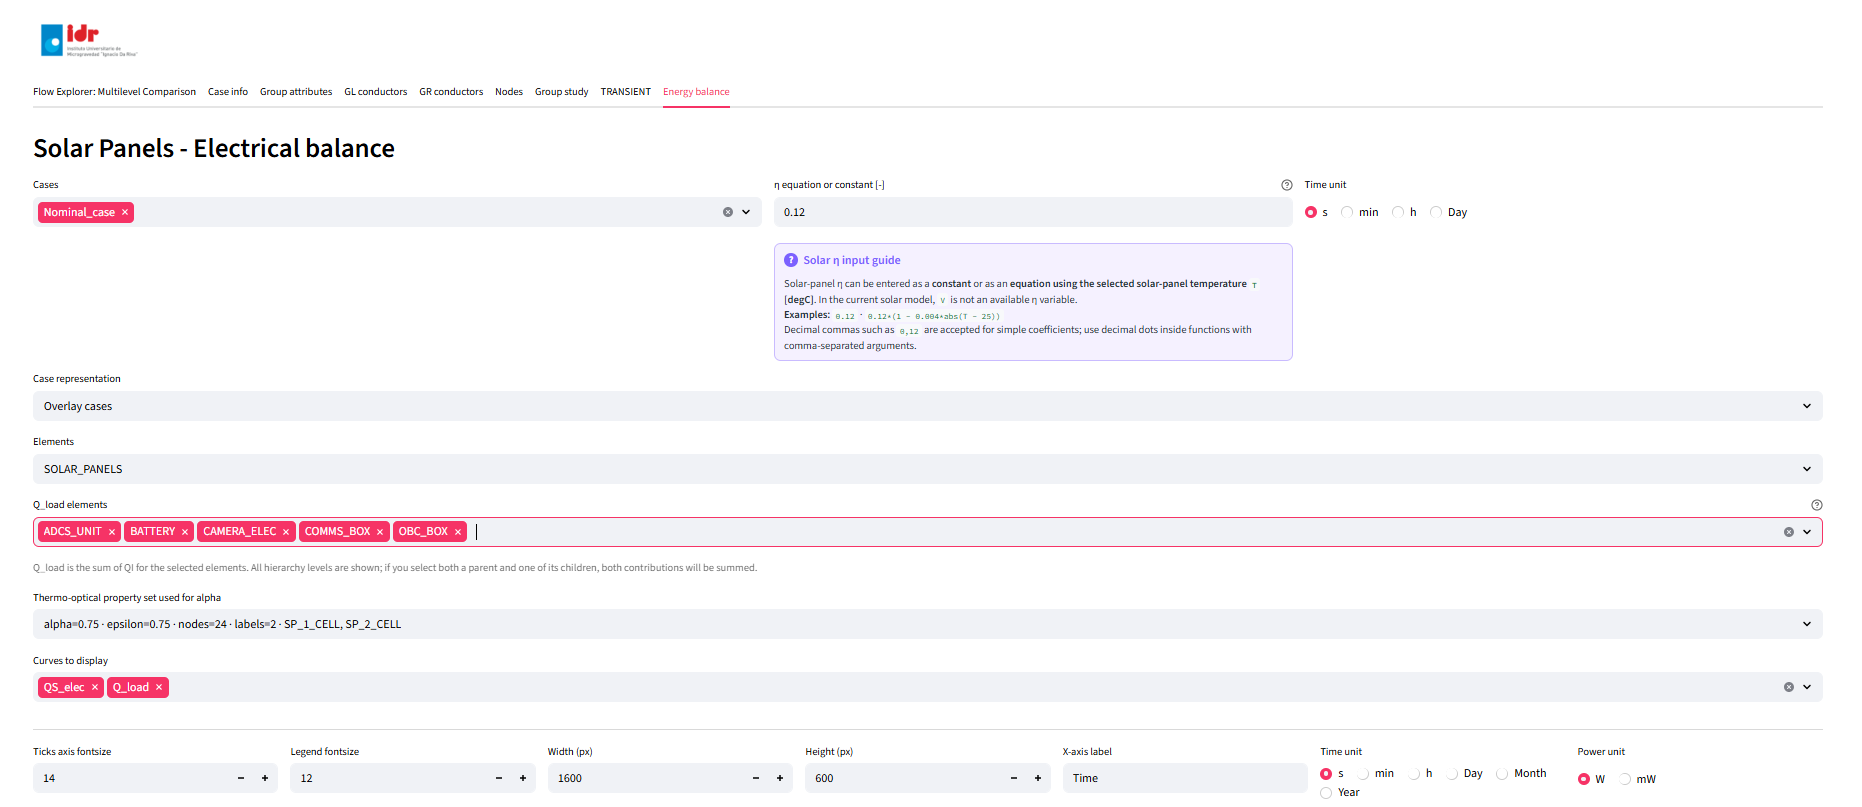
\includegraphics[
        width=0.98\textwidth,
        keepaspectratio
    ]{Figures/08/elec00.png}
    \caption{Configuration of the solar-to-electrical conversion and the
    electrical-load selection.}
    \label{fig:solar_electrical_configuration}
\end{figure}

The graph can display $Q_S$, $Q_{S,\mathrm{elec}}$ and
$Q_{\mathrm{load}}$ on the same time axis. The default selection compares the
available electrical generation with the estimated demand, which directly
reveals the charging and discharging intervals later used by the battery
model. Figure~\ref{fig:solar_electrical_balance_plot} illustrates this output.
Its numerical values only demonstrate the representation available in the tab;
the final case results belong to the subsequent results analysis.

\begin{figure}[H]
    \centering
    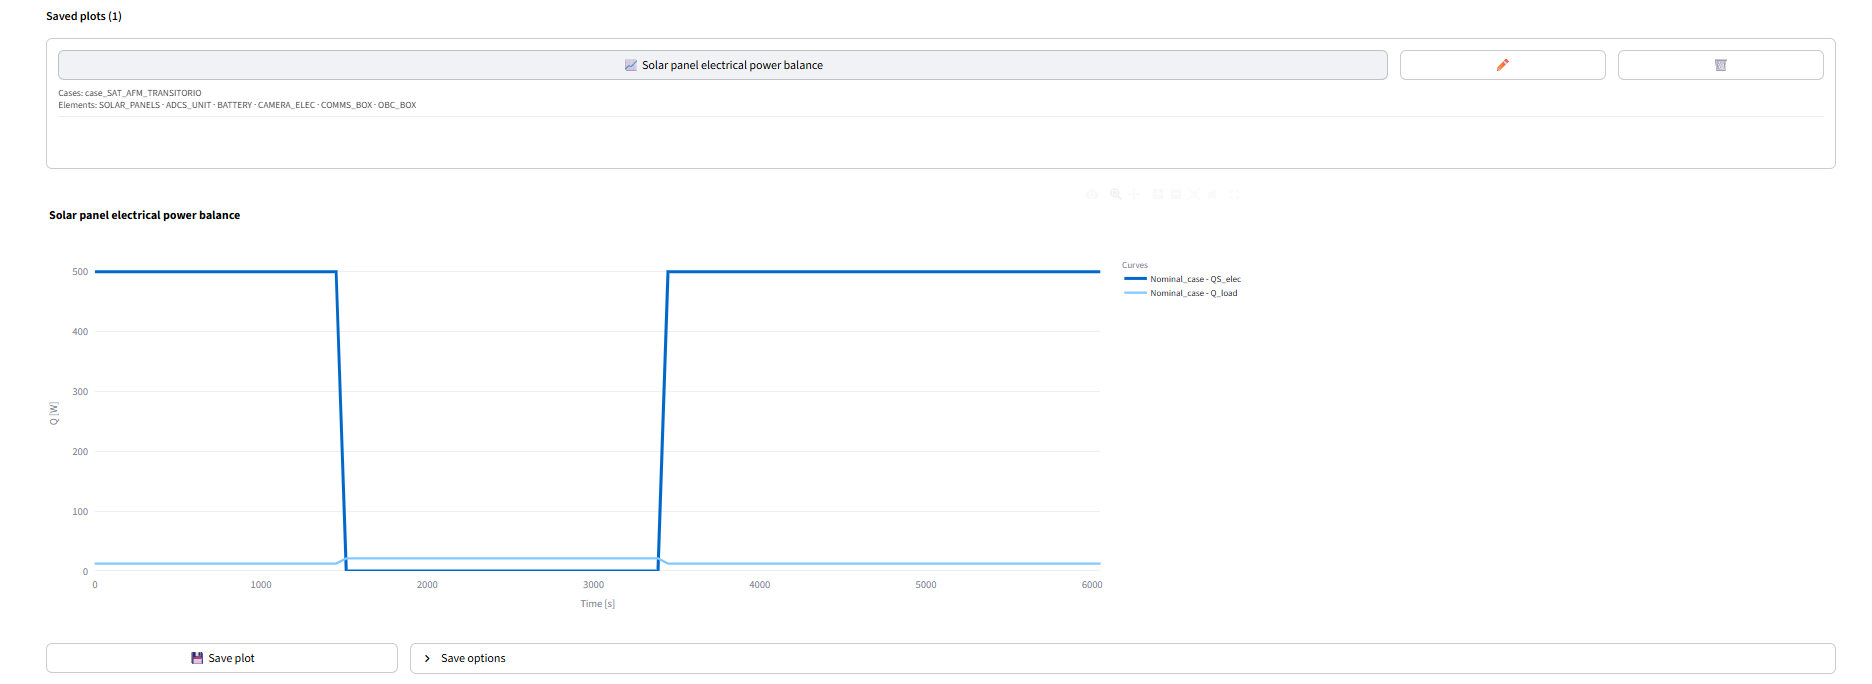
\includegraphics[
        width=0.97\textwidth,
        keepaspectratio
    ]{Figures/08/elec02.png}
    \caption{Illustrative solar-panel electrical balance containing
    $Q_{S,\mathrm{elec}}$ and $Q_{\mathrm{load}}$.}
    \label{fig:solar_electrical_balance_plot}
\end{figure}

An optional calculation table retains the values used at every output instant.
Its columns include $Q_S$, $Q_{S,i}$, $Q_{S,\mathrm{elec}}$,
$Q_{\mathrm{load}}$, $\alpha$, $\alpha_{\mathrm{th}}$ and $\eta$. When the
efficiency depends on temperature, the table also includes the temperature
history supplied to the efficiency expression. This output allows the user to
check the complete conversion before applying the result to the battery.


\section{Battery Model}
\label{sec:battery_model}

The battery calculation starts from the histories generated in the first part
of the tab. At each time interval, solar power first covers the selected load.
The model sends any remaining surplus to the battery and requests discharge
when generation cannot meet the demand. Battery temperature, conversion
efficiencies, voltage limits, internal resistance and charge-control settings
then determine the accepted power and the evolution of the stored energy.

The application recalculates the battery whenever the user changes the solar
element, the $Q_{\mathrm{load}}$ groups, the thermo-optical property, $\alpha$
or the solar-efficiency equation. Consequently, two identical battery
configurations can produce different responses when their upstream
$Q_{S,\mathrm{elec}}$ or $Q_{\mathrm{load}}$ histories differ.


\subsection{Energy-Discharge-Level Basis}
\label{subsec:battery_theoretical_basis}

The battery formulation takes the energy-discharge-level approach proposed by
Porras-Hermoso, Pindado and Cubas as its theoretical basis
\cite{porras2018battery}. Their equivalent-circuit model uses discharged
energy $\phi$ as the main state variable instead of relying only on discharged
ampere-hours. This choice relates the state directly to the exchanged power
and reduces the dependence of the capacity description on a single current
rate.

For a discharge process, the original formulation defines

\begin{equation}
    \phi(t)
    =
    \phi_0
    +
    \int_{t_0}^{t}
    \left[
        V I_d+R_d I_d^2
    \right]\mathrm{d}t,
    \label{eq:porras_discharge_energy_ch8}
\end{equation}

whereas charging decreases the discharged-energy level according to

\begin{equation}
    \phi(t)
    =
    \phi_0
    -
    \int_{t_0}^{t}
    \left[
        V I_c-R_c I_c^2
    \right]\mathrm{d}t.
    \label{eq:porras_charge_energy_ch8}
\end{equation}

Here, $I_d$ and $I_c$ denote the non-negative discharge and charge current
magnitudes, while $R_d$ and $R_c$ represent the corresponding internal
resistances. The terminal voltage follows

\begin{align}
    V_d(\phi,I_d)
    &=
    E_d(\phi)-R_d I_d,
    \label{eq:porras_discharge_voltage_ch8}
    \\
    V_c(\phi,I_c)
    &=
    E_c(\phi)+R_c I_c.
    \label{eq:porras_charge_voltage_ch8}
\end{align}

Porras-Hermoso et al. identify $E_d(\phi)$ and $E_c(\phi)$ from experimental
charge and discharge curves and extend the static equivalent circuit with
additional resistor--capacitor branches for dynamic operation
\cite{porras2018battery}.

The implementation developed for this project retains the energy state, the
separate charge and discharge resistances, and the terminal-voltage relations.
It does not reproduce the experimentally fitted voltage functions or the
dynamic resistor--capacitor branches. Instead, it constructs a generic
piecewise-linear internal-voltage curve $E(\phi)$ from the cell discharge
cut-off, nominal and charge-limit voltages. This reduction keeps the model
configurable when no calibration data exist for a particular flight battery.

Let $C_{\mathrm{pack,Wh}}$ denote the nominal energy capacity and
$E_{\mathrm{st}}(t)$ the stored energy. The implemented discharged-energy
state becomes

\begin{equation}
    \phi(t)
    =
    C_{\mathrm{pack,Wh}}-E_{\mathrm{st}}(t),
    \label{eq:implemented_battery_phi}
\end{equation}

and the reported state of charge follows

\begin{equation}
    \mathrm{SOC}(t)
    =
    100
    \frac{E_{\mathrm{st}}(t)}{C_{\mathrm{pack,Wh}}}.
    \label{eq:implemented_battery_soc}
\end{equation}

The module solves the corresponding relation $P=VI$ to obtain current from the
power requested at each step. It also adds conversion efficiencies, charge and
discharge power limits, temperature-dependent charge derating and a simplified
CC--CV strategy. The resulting curves provide engineering estimates for the
selected configuration rather than an experimentally calibrated prediction of
a specific battery.


\subsection{Thermal Derating and Battery-Pack Configuration}
\label{subsec:battery_configuration}

The first parameter block links the battery calculation with the thermal
solution and defines the physical pack. The \emph{Battery TMD element}
selector identifies the group whose mean temperature represents the battery.
The model uses this history in the charge-derating calculation and in any
charge or discharge efficiency expression that contains $T$.

The lower and upper derating limits define the temperature interval in which
the battery accepts charge. A common ramp margin $m_T$ softens both
transitions. For non-overlapping lower and upper ramps, the implemented factor
can be written as

\begin{equation}
    f_T(T)
    =
    \begin{cases}
        0,
        & T\leq T_{\mathrm{low}},
        \\[0.35em]
        \dfrac{T-T_{\mathrm{low}}}{m_T},
        & T_{\mathrm{low}}<T<T_{\mathrm{low}}+m_T,
        \\[0.9em]
        1,
        & T_{\mathrm{low}}+m_T
          \leq T\leq
          T_{\mathrm{high}}-m_T,
        \\[0.35em]
        \dfrac{T_{\mathrm{high}}-T}{m_T},
        & T_{\mathrm{high}}-m_T<T<T_{\mathrm{high}},
        \\[0.9em]
        0,
        & T\geq T_{\mathrm{high}}.
    \end{cases}
    \label{eq:battery_charge_derating_ch8}
\end{equation}

The factor multiplies the maximum charge current and charge power. A value of
one allows normal charging, a value of zero blocks it, and intermediate values
reduce the accepted surplus linearly. The derating does not limit discharge in
the current implementation.

The cell configuration uses $N_s$ cells in series and $N_p$ parallel strings.
The application obtains the equivalent pack voltages from

\begin{equation}
    V_{x,\mathrm{pack}}
    =
    N_sV_{x,\mathrm{cell}},
    \qquad
    x\in\{\mathrm{cut},\mathrm{nom},\mathrm{chg}\},
    \label{eq:battery_pack_voltages}
\end{equation}

while the charge and nominal energy capacities become

\begin{align}
    C_{\mathrm{pack,Ah}}
    &=
    N_p C_{\mathrm{cell,Ah}},
    \label{eq:battery_pack_ah}
    \\
    C_{\mathrm{pack,Wh}}
    &=
    V_{\mathrm{nom,pack}}C_{\mathrm{pack,Ah}}.
    \label{eq:battery_pack_wh}
\end{align}

The initial SOC fixes the energy available at the first output instant:

\begin{equation}
    E_{\mathrm{st},0}
    =
    \frac{\mathrm{SOC}_0}{100}C_{\mathrm{pack,Wh}}.
    \label{eq:battery_initial_energy}
\end{equation}

Table~\ref{tab:battery_thermal_pack_inputs} summarises every field in this
first parameter block.

\begin{table}[H]
    \centering
    \caption{Battery thermal and pack-configuration inputs.}
    \label{tab:battery_thermal_pack_inputs}
    \small
    \setlength{\tabcolsep}{4pt}
    \renewcommand{\arraystretch}{1.15}
    \begin{tabularx}{\textwidth}{@{}p{0.35\textwidth}X@{}}
        \toprule
        \textbf{Interface field} & \textbf{Role in the calculation} \\
        \midrule

        Battery TMD element &
        Supplies the mean battery temperature used by charge derating and
        temperature-dependent efficiency expressions. \\

        Charge derating lower limit &
        Blocks charging below the selected lower temperature. \\

        Charge derating upper limit &
        Blocks charging above the selected upper temperature. \\

        Charge derating ramp margin &
        Defines the linear transition band beside both charging limits. \\

        Series cells $N_s$ &
        Scales the pack cut-off, nominal and charge-limit voltages. \\

        Parallel strings $N_p$ &
        Scales pack charge capacity and reduces equivalent resistance. \\

        Cell charge capacity &
        Defines the ampere-hour capacity of one cell and, together with $N_p$,
        the pack charge capacity. \\

        Cell discharge cut-off voltage &
        Defines the minimum admissible cell voltage during discharge. \\

        Cell nominal/reference voltage &
        Defines the nominal pack voltage and the conversion from Ah to Wh. \\

        Cell charge voltage limit &
        Defines the upper terminal-voltage limit used during charging. \\

        Initial SOC &
        Sets the stored energy at the start of the transient calculation. \\

        \bottomrule
    \end{tabularx}
\end{table}

Figure~\ref{fig:battery_thermal_pack_configuration} shows the corresponding
controls in the application.

\begin{figure}[H]
    \centering
    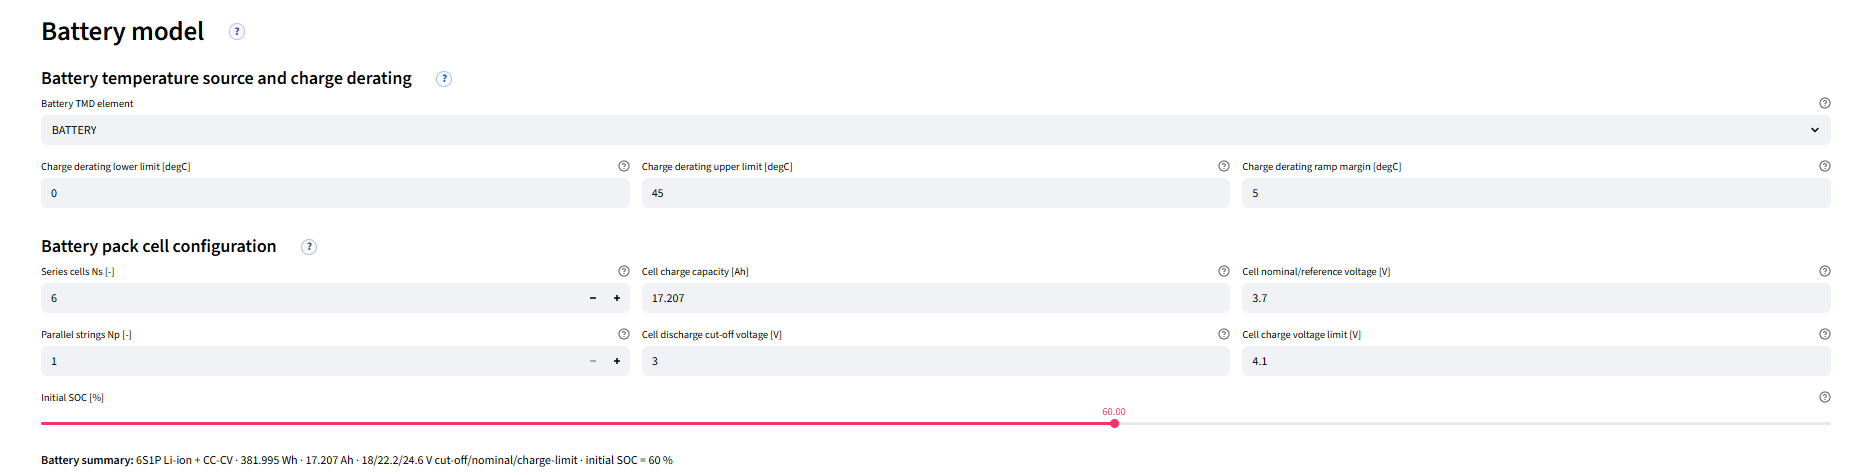
\includegraphics[
        width=0.98\textwidth,
        keepaspectratio
    ]{Figures/08/bat00.png}
    \caption{Battery-temperature reference, charge derating and cell-pack
    configuration.}
    \label{fig:battery_thermal_pack_configuration}
\end{figure}


\subsection{Electrical Parameters and CC--CV Charge Control}
\label{subsec:battery_electrical_parameters}

The second parameter block defines the power-transfer behaviour of the pack.
Charge and discharge efficiencies may use constants or expressions of battery
temperature $T$ and terminal voltage $V$:

\begin{equation}
    \eta_c(t)=f_c\!\left[T_{\mathrm{batt}}(t),V(t)\right],
    \qquad
    \eta_d(t)=f_d\!\left[T_{\mathrm{batt}}(t),V(t)\right].
    \label{eq:battery_efficiency_functions}
\end{equation}

The application requires $0<\eta_c\leq1$ and $0<\eta_d\leq1$. Constants form
the simplest valid expressions. During charge, $\eta_c$ reduces the solar
surplus that reaches the battery terminals. During discharge, $\eta_d$ reduces
the terminal power delivered to the electrical load. The model reports the
remaining difference as conversion loss.

Separate cell resistances retain the charge--discharge asymmetry of the
energy-based equivalent circuit. Their pack values follow

\begin{equation}
    R_{x,\mathrm{pack}}
    =
    R_{x,\mathrm{cell}}
    \frac{N_s}{N_p},
    \qquad
    x\in\{d,c\}.
    \label{eq:battery_pack_resistance_ch8}
\end{equation}

The resistance lowers the discharge terminal voltage and raises the charge
terminal voltage. It also produces the internal loss

\begin{equation}
    P_{\mathrm{loss,int}}(t)
    =
    R I^2(t).
    \label{eq:battery_internal_loss_ch8}
\end{equation}

Maximum charge and discharge powers establish independent caps for both
operating directions. During charging, the CC current ceiling follows the
selected C-rate:

\begin{equation}
    I_{\mathrm{CC,max}}
    =
    C_{\mathrm{rate}}C_{\mathrm{pack,Ah}}.
    \label{eq:battery_cc_current_ch8}
\end{equation}

The temperature factor from Equation~\eqref{eq:battery_charge_derating_ch8}
reduces this ceiling and the maximum charge power. The voltage constraint also
requires

\begin{equation}
    E(\phi)+R_cI_c
    \leq
    V_{\mathrm{chg,pack}}.
    \label{eq:battery_cv_voltage_limit}
\end{equation}

Above the selected SOC threshold $\mathrm{SOC}_{\mathrm{CV}}$, an additional
factor progressively reduces the current:

\begin{equation}
    f_{\mathrm{CV}}(\mathrm{SOC})
    =
    \left[
        \frac{100-\mathrm{SOC}}
        {100-\mathrm{SOC}_{\mathrm{CV}}}
    \right]^{\gamma},
    \qquad
    \mathrm{SOC}\geq\mathrm{SOC}_{\mathrm{CV}},
    \label{eq:battery_cv_taper_ch8}
\end{equation}

where $\gamma$ controls the shape of the reduction. The current remains
subject to the CC limit below this threshold, provided that the solar surplus
and charge-power cap allow it. The model declares practical full charge when
the tapered or voltage-limited current falls below the selected current
threshold; any additional surplus then appears as curtailed solar power.

During discharge, the model limits current through the available stored
energy, the maximum discharge power and the cell discharge cut-off voltage.
Any demand that remains after these restrictions appears as unserved load.

Table~\ref{tab:battery_electrical_inputs} collects every field in this second
parameter block.

\begin{table}[H]
    \centering
    \caption{Battery electrical and CC--CV control inputs.}
    \label{tab:battery_electrical_inputs}
    \small
    \setlength{\tabcolsep}{4pt}
    \renewcommand{\arraystretch}{1.15}
    \begin{tabularx}{\textwidth}{@{}p{0.39\textwidth}X@{}}
        \toprule
        \textbf{Interface field} & \textbf{Role in the calculation} \\
        \midrule

        Charge efficiency equation &
        Defines the fraction of solar surplus transferred towards battery
        charging; it may depend on $T$ and $V$. \\

        Discharge efficiency equation &
        Defines the fraction of terminal discharge power delivered to the
        selected electrical load; it may depend on $T$ and $V$. \\

        Maximum charge power &
        Caps the terminal power accepted from the solar surplus. \\

        Maximum discharge power &
        Caps the terminal power extracted when generation does not cover the
        demand. \\

        Maximum constant-current charge rate &
        Sets the CC current ceiling as a multiple of pack capacity in Ah. \\

        SOC where current reduction towards CV begins &
        Defines the SOC threshold above which the taper factor acts. \\

        Current-reduction shape factor &
        Controls how sharply charge current decreases near full charge. \\

        Charge-complete current threshold &
        Stops charging when the reduced current falls below the selected
        practical limit in the CV region. \\

        Cell discharge internal resistance &
        Determines pack voltage drop and $I^2R$ loss during discharge. \\

        Cell charge internal resistance &
        Determines pack voltage rise and $I^2R$ loss during charge. \\

        \bottomrule
    \end{tabularx}
\end{table}

Figure~\ref{fig:battery_electrical_configuration} shows these controls. The
summary box below the inputs reports the resulting voltage limits, equivalent
pack resistances and an efficiency preview for the current configuration.

\begin{figure}[H]
    \centering
    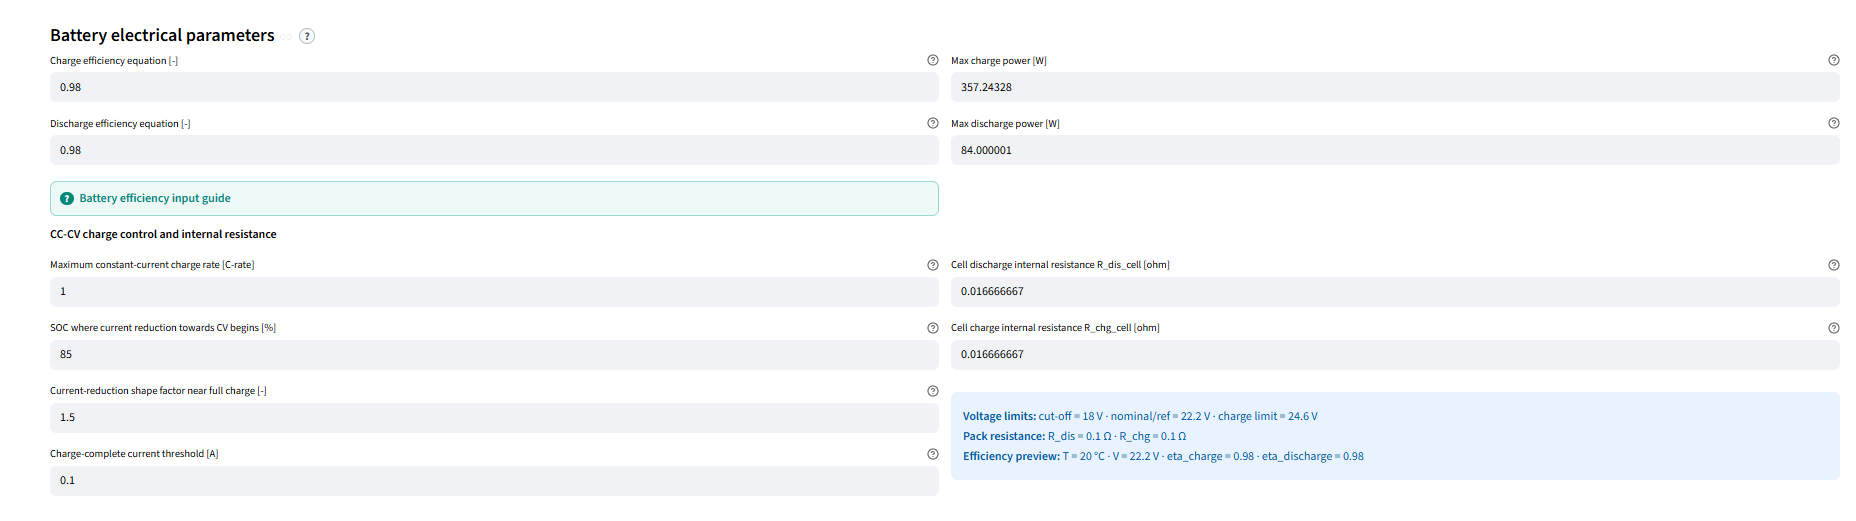
\includegraphics[
        width=0.98\textwidth,
        keepaspectratio
    ]{Figures/08/bat01.png}
    \caption{Battery efficiencies, power limits, internal resistances and
    simplified CC--CV control parameters.}
    \label{fig:battery_electrical_configuration}
\end{figure}


\subsection{Battery Output Curves and Summary Results}
\label{subsec:battery_outputs}

The tab places the graphical outputs immediately after the parameter blocks so
that the user can inspect the effect of each change without leaving the
battery workflow. The first graph shows state of charge throughout the
simulation. Rising segments indicate net storage, falling segments indicate
battery support of the load, and horizontal segments identify intervals in
which the stored energy remains unchanged or reaches an operating limit.

\begin{figure}[H]
    \centering
    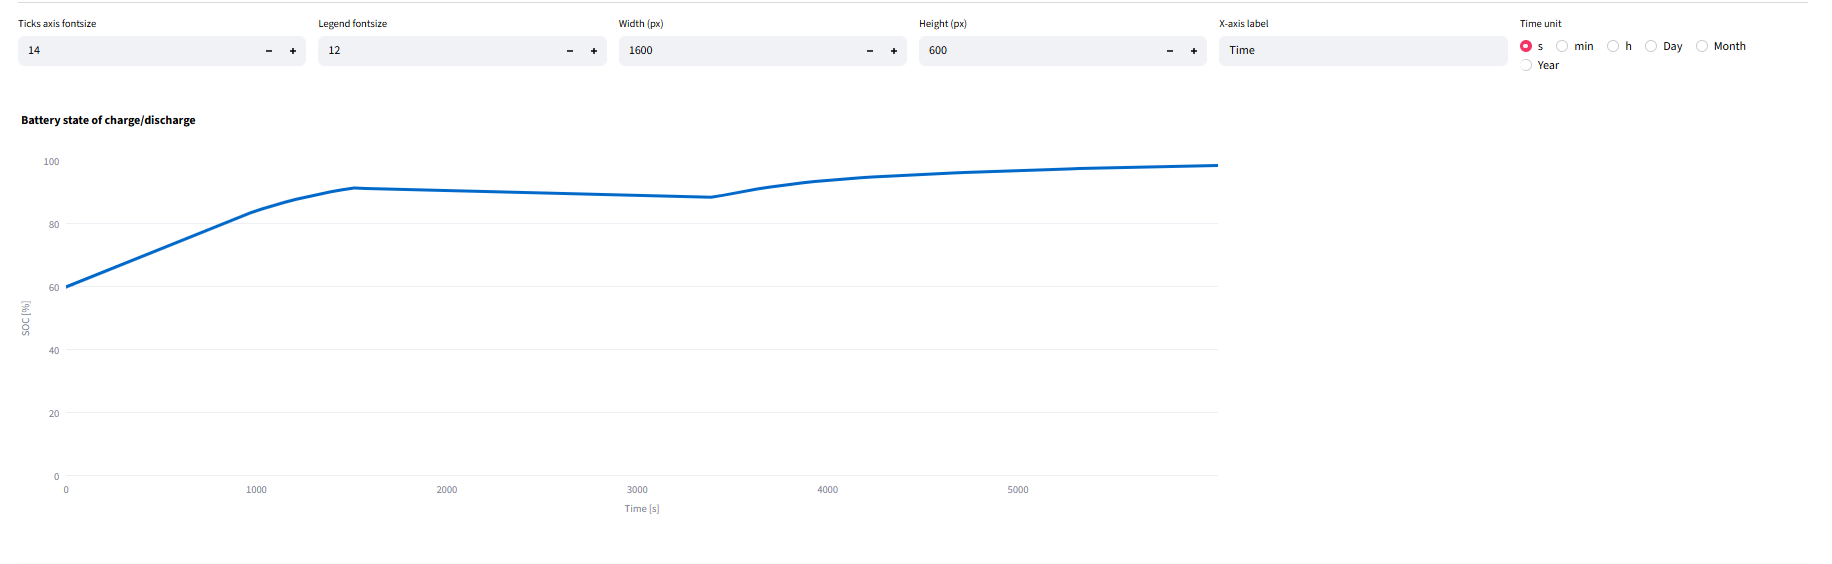
\includegraphics[
        width=0.97\textwidth,
        keepaspectratio
    ]{Figures/08/bat02.png}
    \caption{Illustrative battery state-of-charge history.}
    \label{fig:battery_soc_output}
\end{figure}

The second graph combines terminal voltage with separate non-negative charge
and discharge currents. The left axis represents voltage, while the right axis
represents current. The separation of both current directions avoids relying
on a sign convention in the graphical interpretation, although the detailed
calculation table also retains a signed battery current that is positive in
discharge and negative in charge.

\begin{figure}[H]
    \centering
    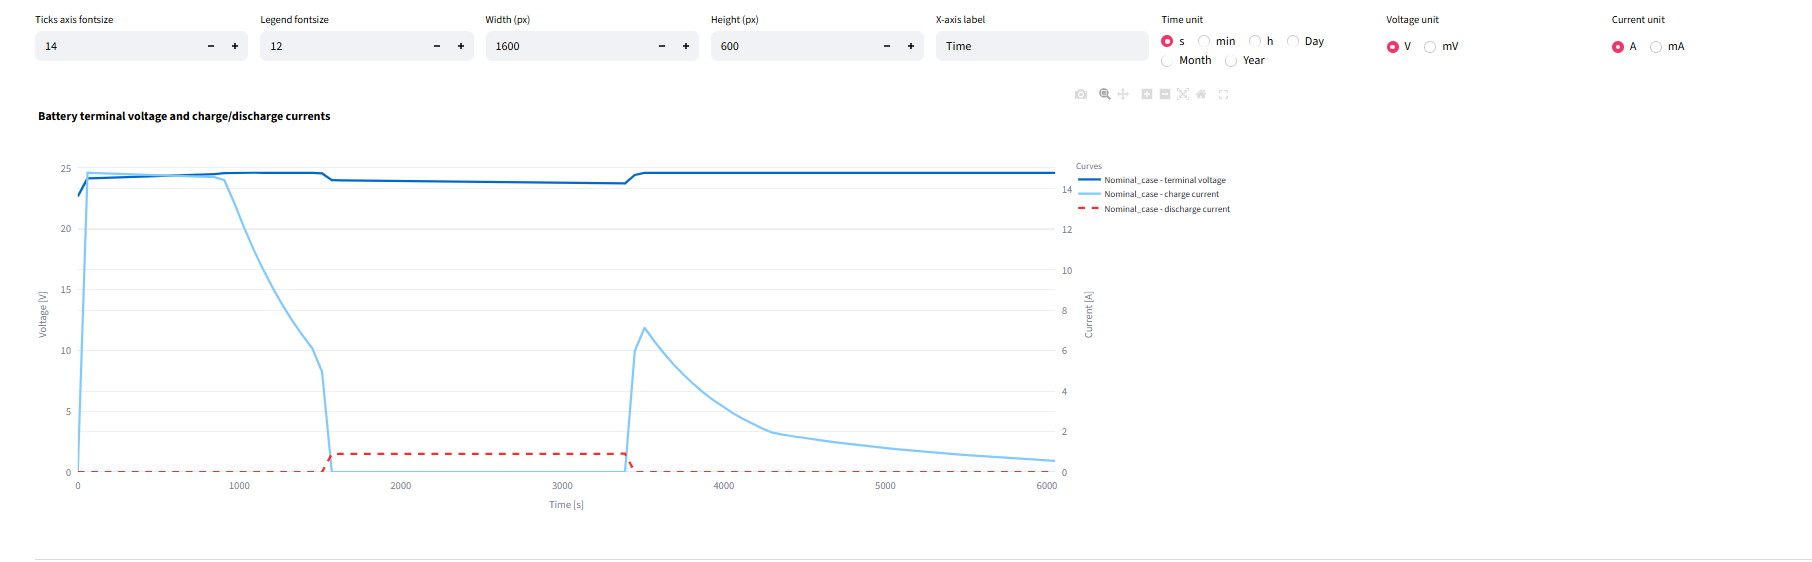
\includegraphics[
        width=0.97\textwidth,
        keepaspectratio
    ]{Figures/08/bat03.png}
    \caption{Illustrative terminal-voltage and charge/discharge-current
    histories.}
    \label{fig:battery_voltage_current_output}
\end{figure}

The third graph connects the thermal result with the battery restrictions. It
places the mean battery temperature on the left axis and the charge-derating,
charge-efficiency and discharge-efficiency factors on the right. This output
shows whether a change in battery behaviour comes from the available power,
the selected efficiency expressions or a temperature-dependent charging
restriction.

\begin{figure}[H]
    \centering
    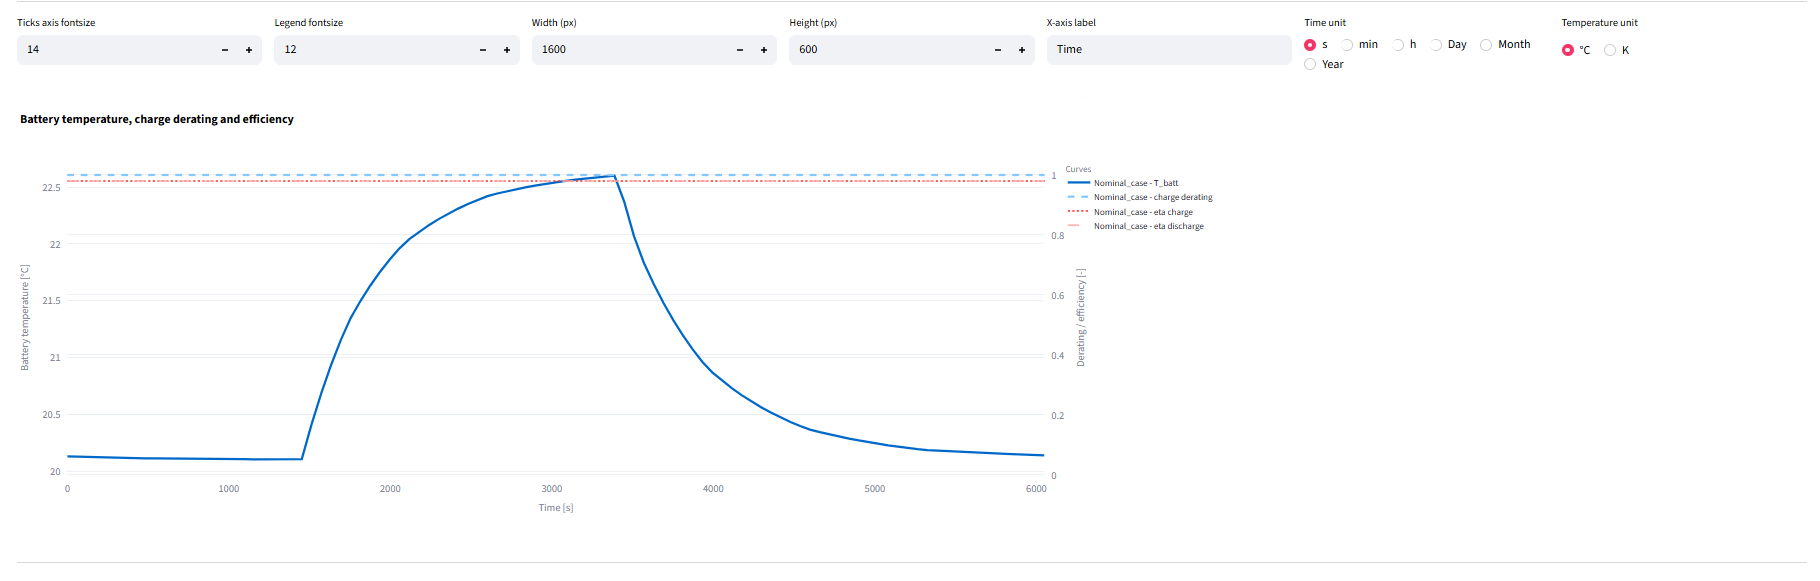
\includegraphics[
        width=0.97\textwidth,
        keepaspectratio
    ]{Figures/08/bat_04.png}
    \caption{Illustrative battery temperature, charge-derating and efficiency
    histories.}
    \label{fig:battery_thermal_output}
\end{figure}

The figures in this subsection demonstrate the form of the available outputs;
they do not yet support conclusions about the final nominal, hot or cold
cases. Their numerical interpretation requires the validated input parameters
and belongs to the results stage of the project.

After the graphs, the battery summary table condenses the complete simulation.
It reports final, minimum and maximum SOC; maximum charge and discharge power;
curtailed solar energy; unserved-load energy; time spent in CC, CV,
solar-limited charge, discharge and voltage-limited discharge; minimum and
maximum battery temperature; minimum derating factor; total derated time; and
the ranges of charge and discharge efficiency.

A second, optional calculation table retains the values at every output
instant. Its principal columns include
$Q_{S,\mathrm{elec}}$, $Q_{\mathrm{load}}$, direct solar supply, surplus,
deficit, charge and discharge powers, terminal and internal voltages, charge
and discharge currents, SOC, $\phi$, stored energy, efficiencies, curtailed
solar power, unserved load, internal and conversion losses, battery
temperature, derating factor and operating phase. Together, the graphs and
tables connect the selected thermal case with the complete electrical and
battery post-processing sequence.
